% Options for packages loaded elsewhere
\PassOptionsToPackage{unicode}{hyperref}
\PassOptionsToPackage{hyphens}{url}
%
\documentclass[
]{article}
\usepackage{lmodern}
\usepackage{amssymb,amsmath}
\usepackage{ifxetex,ifluatex}
\ifnum 0\ifxetex 1\fi\ifluatex 1\fi=0 % if pdftex
  \usepackage[T1]{fontenc}
  \usepackage[utf8]{inputenc}
  \usepackage{textcomp} % provide euro and other symbols
\else % if luatex or xetex
  \usepackage{unicode-math}
  \defaultfontfeatures{Scale=MatchLowercase}
  \defaultfontfeatures[\rmfamily]{Ligatures=TeX,Scale=1}
\fi
% Use upquote if available, for straight quotes in verbatim environments
\IfFileExists{upquote.sty}{\usepackage{upquote}}{}
\IfFileExists{microtype.sty}{% use microtype if available
  \usepackage[]{microtype}
  \UseMicrotypeSet[protrusion]{basicmath} % disable protrusion for tt fonts
}{}
\makeatletter
\@ifundefined{KOMAClassName}{% if non-KOMA class
  \IfFileExists{parskip.sty}{%
    \usepackage{parskip}
  }{% else
    \setlength{\parindent}{0pt}
    \setlength{\parskip}{6pt plus 2pt minus 1pt}}
}{% if KOMA class
  \KOMAoptions{parskip=half}}
\makeatother
\usepackage{xcolor}
\IfFileExists{xurl.sty}{\usepackage{xurl}}{} % add URL line breaks if available
\IfFileExists{bookmark.sty}{\usepackage{bookmark}}{\usepackage{hyperref}}
\hypersetup{
  pdftitle={Aveage Annualized Loss in R},
  pdfauthor={Niko T Todorov},
  hidelinks,
  pdfcreator={LaTeX via pandoc}}
\urlstyle{same} % disable monospaced font for URLs
\usepackage[margin=1in]{geometry}
\usepackage{graphicx,grffile}
\makeatletter
\def\maxwidth{\ifdim\Gin@nat@width>\linewidth\linewidth\else\Gin@nat@width\fi}
\def\maxheight{\ifdim\Gin@nat@height>\textheight\textheight\else\Gin@nat@height\fi}
\makeatother
% Scale images if necessary, so that they will not overflow the page
% margins by default, and it is still possible to overwrite the defaults
% using explicit options in \includegraphics[width, height, ...]{}
\setkeys{Gin}{width=\maxwidth,height=\maxheight,keepaspectratio}
% Set default figure placement to htbp
\makeatletter
\def\fps@figure{htbp}
\makeatother
\setlength{\emergencystretch}{3em} % prevent overfull lines
\providecommand{\tightlist}{%
  \setlength{\itemsep}{0pt}\setlength{\parskip}{0pt}}
\setcounter{secnumdepth}{-\maxdimen} % remove section numbering

\title{Aveage Annualized Loss in R}
\author{Niko T Todorov}
\date{12/07/2020}

\begin{document}
\maketitle

\hypertarget{introduction}{%
\subsection{Introduction}\label{introduction}}

FEMA collects natural hazards -- flood, hurricane, earthquake, tsunami
-- for deterministic events -- such as Katrina, Sandy, Harvey
hurricanes, Northridge earthquake to name a few -- and probabilistic
from 10 year to 1000 year probability of occurance, which we will call
return periods (RPs). This AALinR module assumes the existance of
several (more than 1) probabilistic data points, for the time being, in
the predefined RPs {[}10, 25, 50, 100, 200, 500, 1000{]}, but in the
future extendable to any random RP. The import data in space-delimited
format is: (ID RP Loss).

The AALinR will produce the Average Annualized Loss using Riemann
numerical integration midpoint method.

\hypertarget{current-assumptions}{%
\subsection{Current assumptions}\label{current-assumptions}}

\begin{itemize}
\tightlist
\item
  RPs must be one of {[}10, 20, 50, 100, 200, 500, 1000{]}.
\item
  No missing RP or outlier data detection.
\end{itemize}

\hypertarget{future-enhancements}{%
\subsection{Future enhancements}\label{future-enhancements}}

\begin{itemize}
\tightlist
\item
  Random RP losses.
\item
  missing, erroneous, outlier data detection/correction.
\end{itemize}

\hypertarget{faq}{%
\subsection{FAQ}\label{faq}}

Q: How is AAL different from the 1 return period (RP) loss? A: The AAL
is the mean value of a loss exceedance probability (EP) distribution. It
is the expected loss per year, averaged over many years. The one-year
return period loss has 100\% chance of occurance and is expected to be
at least equaled every year.

Q: What is the RP loss relationship w.r.t. the probability of occurance?
A: The RP loss has inverse relationship w.r.t. probability of occurance.
For example 100-year RP loss is said to equal 1/100 or 1\% chance.
Similarly, 10-year \textasciitilde{} 1/10 or 10\% chance, 25-year
\textasciitilde{} 1/25 or 4\% chance, 500-year \textasciitilde{} 1/500
or 0.2\% chance of occurance.

Q: Why AAL? A: because it is a good measure for relative natural hazards
risk of a geographic area.

Q: What is the ID? A: it could be a Census Block (CB), Census Tract
(CT), County (CO), State (ST), or individual buildings, for which may
have to use Google Plus codes.

\hypertarget{computational-modeling-and-biodiversity}{%
\subsubsection{Computational Modeling and
Biodiversity}\label{computational-modeling-and-biodiversity}}

Most biological functional systems are complex. In these systems,
variation in morphology and behavior leads to differences in performance
at a variety of tasks, influencing individual fitness. Because
functional systems are complex, variation in these input parameters do
not have linear consequences to functional performance or fitness.
Complexity often results in mechanical equivalence, or ``many-to-one
mapping," in which different combinations of parameters lead to the same
or similar values of performance {[}1{]}. In these ways, complexity may
be a fundamental driver of morphological diversity {[}1{]}.

Therefore, understanding the connection between morphological and
kinematic (input parameters) variation and functional performance
(output) is key to understanding the evolution and diversity of complex
functional systems {[}4{]}. Performance could be highly sensitive to
variation in input parameters, meaning small changes in input could lead
to disproportionately large changes in performance. On the other hand,
performance could be insensitive to variation, leading to little change.
Additionally, parameters rarely act independently, so understanding the
system as a whole is important.

Computational modeling provides a solution to this problem. Complexity
can be examined with models by decoupling parameters. Modeling can
create structures and kinematics not naturally possible to isolate and
control in biological systems, giving us a greater ability to test
hypotheses of function. They can also explore variation by sampling a
greater parameter space than what exists naturally in morphological
diversity, providing a way to create full performance landscapes. Models
can examine many-to-one mapping, genetic drift, and other synergies
through output analysis in ways that traditional experimentation and
morphometrics cannot {[}6{]}.

However, many computational models are limited by qualitative analysis
techniques {[}10{]}. The difficulty in analyzing multi-parameter,
multi-variable computational models curtails our ability to understand
the practical implications of changing one parameter over another since
qualitative analyses cannot directly compare the relative contributions
of parameters to system performance. Typical analyses involve
qualitative measures of performance by changing over only one variable
(parameter sweeping), which can neglect effects of many-to-one mapping
and synergy between parameters.

As a step towards connecting modeling and diversity of form, we apply a
quantitative sensitivity analysis through uncertainty quantification
(UQ) of a computational fluid dynamic (CFD) model of functional
performance. UQ can help resolve these issues and broaden the impact of
computational modeling on studies of evolution. Quantitative sensitivity
analyses can improve our understanding of: 1) the effects of
biologically important variation on the system, and 2) the relative
importance of parameters that should be closely assessed. In addition,
UQ can be used to make conclusions about the variation in existing
morphological diversity (based on sensitivity analyses) and validate and
improve models when compared to real measurements.

\hypertarget{uncertainty-quantification}{%
\subsubsection{Uncertainty
Quantification}\label{uncertainty-quantification}}

Uncertainty quantification (UQ) studies the uncertainty in the
deterministic modeling process of a physical system, and therefore makes
it possible to provide more accurate, precise, and reliable model
predictions. UQ accomplishes this by analyzing the effects of known
variation of input parameters on the model's output.

Uncertainty in a model's input is normally represented using probability
measures and uncertainty quantification frameworks that have been well
established based on probability theory. Probability distribution
functions (PDFs) represent the uncertainty in input parameters based on
measured value ranges. Then the uncertainty in the model output can be
quantified using its distribution or statistics instead of relying on a
single deterministic value.

A common way to obtain this mathematical representation of uncertainty
output is by using Monte Carlo (MC) method, which draws samples from a
distribution of the deterministic model's input parameters, implements
the simulations at the drawn samples, and then provides the
corresponding samples (consequently the empirical distribution) of the
model output. MC method is easy to implement and straightforward to
understand. However, it can be computationally expensive since it may
require a large number of full simulations to achieve a desired accuracy
due to its slow convergence.

To represent the uncertainty in the output more efficiently than other
techniques (i.e.~Monte Carlo), one may construct a computationally
cheaper surrogate of the input parameter space to approximate the full
CFD model output. Generalized polynomial chaos (gPC) expansion method is
an efficient way to construct this approximation. The gPC method expands
the square integrable random functions in terms of orthogonal
polynomials of the random variables. Hermite polynomials are first used
to represent Gaussian processes based on the homogeneous chaos theory
{[}11{]}, then extended to the Askey scheme with different types of
orthogonal polynomials for different random functions/processes
{[}12{]}. By corresponding the PDF of random variables to the weighting
function of the orthogonal polynomials from the Askey scheme, the gPC
method reaches fast convergence for smooth functions.

Compared to Monte Carlo method, the gPC method requires far fewer model
simulations to reach the same accuracy, and its efficiency can be orders
of magnitude higher {[}13{]}. Because of the computational demands of
CFD modeling, the gPC method represents a huge improvement in our
ability to study these complex systems. Therefore, the gPC method is
adopted in our current work.

Based on the gPC expansion, global sensitivity analysis using Sobol
indices can be implemented {[}15{]}. Sensitivity analysis studies the
impact of different stochastic input variables on the quantity of
interest, which helps to understand the important factors in functional
performance and possibly reduce the complexity of the physical system
{[}16{]}. The Sobol index (SI) is an important sensitivity measure based
on analysis of variance (ANOVA) decomposition {[}17{]}. It is defined as
the ratio of the variance in the sub-dimensional problem to the total
variance of the full-dimensional problem. The higher the SI ratio is,
the more important the set of input parameters in that sub-dimensional
space is.

In this study, we begin with a relatively simple model of a complex,
biological system as proof of principle: peristaltic pumping in a simple
racetrack circulatory system. We use the gPC expansion method to
construct a surrogate of the input parameter space of peristaltic
pumping and implement sensitivity analysis to determine how input
variation in parameters impacts functional performance.

\hypertarget{driving-circulatory-flow-with-peristalsis}{%
\subsubsection{Driving Circulatory Flow with
Peristalsis}\label{driving-circulatory-flow-with-peristalsis}}

Driving fluid with contractions of valveless tubes is widespread in
animals and serves a variety of purposes, including pumping lymph and
other fluids {[}19{]}, driving fluid exchange in respiratory systems
{[}23{]}, and driving circulatory systems {[}27{]}. Within the Chordata,
valveless, tubular pumps (hearts) drive blood flow within circulatory
systems in tunicates, cephalochordates, and embryonic vertebrates
{[}28{]}. In vertebrate embryos, a valveless, tubular heart is the first
organ to function and the flow it generates impacts the development of
all other organs {[}30{]}.

Broadly, peristaltic pumps are classified as valveless, tubular pumps.
Valveless, tubular pumps in animals are hollow, muscular tubes that
produce flow through contractions of the walls. Such contractions reduce
the diameter of the tube that drives fluid inside the lumen of the tube.
Valveless, tubular pumps can be driven by peristalsis (rhythmic
contractions of muscles within the walls of the tube that are propagated
down the length of the tube) or Liebau pumping (where contractions at
certain points on the tube travel in passive waves dictated by the
material properties of the tube itself) {[}31{]}. The direction of the
flow inside the tube is controlled only by aspects of the pumping
kinematics (e.g.~the direction of the contracting wave), not by any
physical means (e.g.~one-way valves).

There is some debate as to whether the pumping mechanisms of tubular,
valveless hearts in animals best fits with the definition of peristalsis
or Liebau pumping (for recent discussions, see {[}31{]}). Recent work
has suggested that peristalsis or some peristalsis-like mechanism bests
fits the available data and theoretical understanding of each mechanism
{[}32{]}. Here, we simplify the situation by focusing exclusively on
peristaltic pumping by tubular hearts.

Despite their simple outward appearance, pumping by peristaltic hearts
is a complicated functional system. This mechanical system has a variety
of parameters, including:

\begin{itemize}
\tightlist
\item
  \emph{Morphology of the heart.} Parameters associated with morphology
  which possibly influence flow include the tube's relative resting
  diameter and length {[}32{]}, the mechanical properties of the
  myocardium and surrounding structures {[}37{]}, and the resistivity of
  the circulatory system. These morphological features show variation
  among animals within the Chordata {[}27{]}, but the role of such
  features in functional performance is not well understood.
\item
  \emph{Kinematics of tube compression.} The frequency of compressions
  can have a complicated, non-linear relationship with flow speeds
  {[}39{]}. Compression ratio, the percent occlusion of the tube, can
  affect flow speeds in non-linear ways {[}32{]}. Feedback between the
  action potentials and mechanical properties of the myocardium also
  impact flow features {[}34{]}.
\item
  \emph{Size and scaling.} Fluid flow undergoes a critical transition
  between small sizes and speeds, where the viscosity of fluid damps out
  unsteady effects, to large sizes and speeds, where inertia is
  relatively more influential to the character of fluid flow than
  viscosity and unsteady effects are important. For pulsatile flow, a
  ratio between inertial and viscous forces is called the Womersley
  number (\(Wo\)) and helps to define the transition (at
  \(Wo\approx1\)): \begin{equation}
  Wo = d\sqrt{\frac{f \rho}{\mu}},
  \label{Wo}
  \end{equation} where \(f\) is the frequency of the pulse, \(d\) is the
  resting diameter of the tube, \(\mu\) is fluid dynamic viscosity, and
  \(\rho\) is fluid density. Embryonic vertebrates possess circulatory
  systems that grow through this transitional range with tubular hearts
  that transform into chambered hearts with valves during development.
  Other groups of animals explore size through evolutionary time,
  retaining a tubular heart throughout their lives.
\end{itemize}

Performance of hearts can be assessed in several ways. Volume flow rate
may be an important performance output, as flow produced by the heart
transports key nutrients and waste {[}40{]}. However, this fluid
transport comes at a cost, as work must be done by the myocardium to
force viscous fluid through a resistive circulatory system. It is likely
that performance trade-offs exist in this system, and these trade offs
are inevitably mediated by variation in input parameters.

Analytical models and approximations of peristalsis have been used to
describe many aspects of peristaltic transport, including the average
flow as a function of the wave speed and contraction amplitude {[}41{]}.
These models typically assume contraction amplitudes are small, inertia
is negligible, there is no flow in the radial direction, and/or any
effects of elastic storage are negligible. Furthermore, metrics such as
the cost of transport and the amount of mixing are not readily
obtainable. Few, if any, studies have examined this flow in the context
of resistive circulatory systems, a key evolutionary development in
vertebrate circulation.

Computational modeling of flow produced by valveless, tubular hearts has
improved our understanding of biological pumps, since many of the
assumptions made in analytical models are not required and metrics such
as the cost of transport and mixing dynamics can be readily quantified.
These models have also helped clarify the mechanism of pumping of hearts
such as those of vertebrate embryos {[}32{]}, as well as our
understanding of other important developmental morphological changes
including the development of cardiac cushions, the presence of
trabeculae, and the presence of blood cells {[}45{]}.

\hypertarget{study-objectives}{%
\subsubsection{Study Objectives}\label{study-objectives}}

In the current work, we implement UQ techniques to explore peristalsis
in a circulatory system using the immerse boundary method, a
computational fluid dynamics (CFD) model. We present two mechanisms of
peristalsis in this work: peristalsis driven by opposing sine waves and
peristalsis driven by opposing sharp, Gaussian peaks. Our aims are to
(1) demonstrate the effectiveness of the UQ method for assessing the
impact of input variation on a functional system modeled
computationally; (2) assess the impacts of elastic interactions using
two models of peristalsis; and (3) use the results and sensitivity
analyses to make prediction of morphology and kinematic combinations
that make especially effective pumps.

We constructed two-dimensional models of peristalsis in a heart tube
which drive flow through a closed racetrack circulatory system. We then
constructed a surrogate to replace the full input space of the CFD model
using gPC expansion. Using sensitivity analysis, we explore the
interactive effects on performance outputs (flow in the system, work,
and cost of transport) of morphology, kinematics, and size through three
input parameters: the dimensionless Womersley number \(Wo\) (eq.
\ref{Wo}), compression ratio of the tube \(CR\), and compression
frequency \(f\) with constant wave speed. Based on these results, we
make conclusions about the diversity of these parameters in extant
groups of animals with peristaltically driven circulatory flow.

\hypertarget{materials-and-methods}{%
\subsection{Materials and Methods}\label{materials-and-methods}}

\hypertarget{computational-model-of-peristalsis}{%
\subsubsection{Computational Model of
Peristalsis}\label{computational-model-of-peristalsis}}

\hypertarget{immersed-boundary-method}{%
\paragraph{Immersed Boundary Method}\label{immersed-boundary-method}}

The models of peristalsis (presented in {[}32{]}) were implemented using
the immersed boundary method (IBM) and with the C++ library Immersed
Boundary with Adaptive Mesh Refinement (IBAMR) {[}48{]}. IBM allows a
direct, numerical simulation of the Navier-Stokes equations of fluid
flow interacting with flexible boundaries moving either freely or with
preferred motion. IBAMR incorporates adaptive mesh refinement, which
allows the Eulerian grid on which the Navier-Stokes equations are solved
to be rougher away from the boundaries and finer close to boundaries to
save computational resources. Additional details of the IBM are located
in the supplemental information to this paper.

\begin{figure}
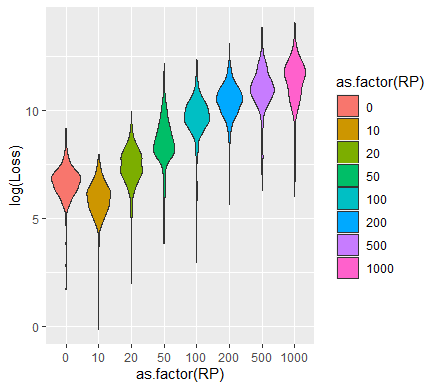
\includegraphics[width=1\linewidth]{../fig/Rplot} \caption{Racetrack model showing adaptive meshing. Full racetrack showing the $R_{top}$ and $R_{bot}$ used to generate prescribed motion in red and adaptive meshing of domain: roughest mesh (32 x 32 grid) in dark blue, intermediate mesh (16 x 16 grid) in teal, and finest mesh (8 x 8 grid) in gold, black box highlights inset a. Inset a: close up of region including part of the tube and racetrack showing meshes, black box highlights inset b. Inset b: close up of tube showing relation of finest mesh and target points of the racetrack. }\label{fig:grid-fig}
\end{figure}

The circulatory model consisted of a racetrack that was effectively made
rigid through the use of tether points with an inner lumen, two straight
sections connected by two curved regions, and a moving region at the
bottom of the racetrack, representing the heart tube that moved with a
preferred motion. The racetrack design was used to stay consistent with
past designs for easier comparison to other analyses {[}49{]}.

The elastic region had a 4:1 length:diameter ratio with the inner 3/4 of
the tube length consisting of points tethered to target points, which
drove the preferred peristaltic motion (Fig. \ref{fig:grid-fig}). The
rest of the racetrack were tethered to target points which remained
still throughout the simulations. Target point stiffness (\(k_{targ}\))
was chosen as 30.0 to remain consistent with the model in {[}32{]}.

The force equation used to drive peristalsis in the model is:
\begin{equation}
\mathbf{f}(r,t) = k_{targ}(\mathbf{Y}(r,t) - \mathbf{X}(r,t))
\label{eq:f}
\end{equation} where \(\mathbf{Y}(r,t)\) is the preferred position of
the boundary. Only the preferred motion of the boundary in each model of
peristalsis differed. Each model of driving peristalsis is described
below.

\hypertarget{opposing-sine-wave-peristalsis-model}{%
\paragraph{Opposing sine-wave peristalsis
model}\label{opposing-sine-wave-peristalsis-model}}

The sine-wave model defines the motion of the boundary as two opposing
sine waves: \begin{equation}
y_{top,bot} = R_{top,bot} \pm A \sin(2\pi f t+ 2\pi cx_t)
\label{eq:sinewaves}
\end{equation} where \(f\) is the compression frequency, \(c\) is the
compression-wave speed (held constant throughout the study at a
non-dimensional speed of 3.0), \(A\) is the amplitude of the
contraction, and \(x_t\) is the horizontal distance from the beginning
of the prescribed motion section. The compression ratio gives the
percent occlusion and is equal to \(2A\). The peristaltic waves created
by Eq.\textasciitilde{}\ref{eq:sinewaves} propagated from left to right,
therefore driving fluid flow counter-clockwise in the lumen of the
racetrack. The stiffness of the boundary and target point stiffness
(\(k_{targ}=30.0\)) allowed for very little independent elastic motion
in the peristaltic region of the tube.

For additional details on the opposing sine-wave peristalsis model, see
{[}32{]}.

\hypertarget{opposing-gaussian-peak-peristalsis-model}{%
\paragraph{Opposing Gaussian-peak peristalsis
model}\label{opposing-gaussian-peak-peristalsis-model}}

The pinch model defines the motion of the boundary as two sharp,
Gaussian peaks, with the remainder of the boundary being free to flex
with little restriction by the target points: \begin{equation}
y_{top,bot} = R_{top,bot} \pm A\exp((-0.5(x_t-\gamma)/\sigma)^2)
\label{eq:gaussianwaves}
\end{equation} Where \(\gamma\) is the position of the pinch on the
x-axis of the center of the tube and \(\sigma\) is the width of the
pinch. The pinch was advanced by altering \(\gamma\) depending on the
time step of the simulation. For the points within the region of the
Gaussian wave, the target point stiffness was chosen to be extremely
stiff (\(k_{targ}=2500\)) so that the target points adhered closely to
the programmed waveform. Outside the peak region, the target points were
tethered very loosely (\(k_{targ}=0.7\)) with a spring constant about
two orders of magnitude stiffer to allow for elastic interactions
between fluid and the heart tube.

\hypertarget{analysis-of-flow-and-pressure-fields}{%
\subsubsection{Analysis of Flow and Pressure
Fields}\label{analysis-of-flow-and-pressure-fields}}

Several calculations of non-dimensional fluid flow and pressure were
made for each simulation in VisIt 2.9.1 {[}50{]} and \emph{R} {[}51{]},
similar to the analyses in {[}32{]}. Positive flow speeds indicate fluid
motion in the counter-clockwise direction in the racetrack, the same
direction as the traveling peristaltic wave. All values presented in the
analysis are dimensionless, and more information about
nondimensionalizing values can be found in the supplemental information
to this paper.

At each time step in the simulation, the magnitude of dimensionless
fluid velocity was recorded and then spatially averaged across each area
to find \(|\mathbf{u'}|\) across four rigid sections of the racetrack:
the upper position, a connecting vertical position, the inflow region
(vena cava) and outflow region (aorta). The mean speeds
\(|\mathbf{u'}|\) were then temporally averaged to find the average flow
speed across each simulation (\(U_{avg}\)). The maximum value of flow
speed, \(\mathbf{u'_{m}}\), was also taken at each time step, and the
maximum of these in a simulation represents the peak flow speed
(\(U_{peak}\)).

Non-dimensional pressure was also recorded for each time step of the
simulation and spatially averaged at each time step near the inflow area
(vena cava position) and the outflow area (aorta position) of the
elastic region. For each simulation, the vena cava and aorta positions'
pressures were averaged temporally to find \(p_{in}\) and \(p_{out}\),
respectively. Each inflow pressure was subtracted from the outflow
pressure at each time step to find their difference, and these
differences were averaged over simulation time to find \(\Delta P\).

Volume flow rate was calculated using the velocity profile across the
upper position of the racetrack for each simulation. At each time step
during a simulation, the velocities were sampled across the diameter of
the tube to create a velocity profile across the tube. Each value was
then used to calculate the volume of a concentric ring of fluid that
passed through the tube during the time step based on the velocity at
that position in the tube. These rings were then summed to find the
volume flow rate at that time step, then these volume flow rates were
averaged temporally to find the average volume flow rate of the
simulation, \(Q\).

\hypertarget{results}{%
\subsection{Results}\label{results}}

\hypertarget{references}{%
\subsection*{References}\label{references}}
\addcontentsline{toc}{subsection}{References}

\hypertarget{refs}{}
\leavevmode\hypertarget{ref-Wainwright:2005}{}%
1. Wainwright PC, Alfaro ME, Bolnick DI, Hulsey CD. 2005 Many-to-one
mapping to form to function: A general principle in organismal design?
\emph{Integr. Comp. Biol.} \textbf{45}, 256--262.

\leavevmode\hypertarget{ref-Anderson:2015}{}%
2. Anderson P, Patek S. 2015 Mechanical sensitivity reveals evolutionary
dynamics of mechanical systems. \emph{Proceedings of the Royal Society
of London B: Biological Sciences} \textbf{282}, 20143088.

\leavevmode\hypertarget{ref-Wainwright:2007}{}%
3. Wainwright PC. 2007 Functional versus morphological diversity in
macroevolution. \emph{Annual Review of Ecology, Evolution, and
Systematics}, 381--401.

\leavevmode\hypertarget{ref-Munoz:2019}{}%
4. Muñoz MM. 2019 The evolutionary dynamics of mechanically complex
systems. \emph{Integrative and Comparative Biology} \textbf{59},
705--715.

\leavevmode\hypertarget{ref-Polly:2016}{}%
5. Polly PD, Stayton CT, Dumont ER, Pierce SE, Rayfield EJ, Angielczyk
KD. 2016 Combining geometric morphometrics and finite element analysis
with evolutionary modeling: Towards a synthesis. \emph{Journal of
Vertebrate Paleontology} \textbf{36}, e1111225.

\leavevmode\hypertarget{ref-Koehl:2003}{}%
6. Koehl MAR. 2003 Physical modeling in biomechanics. \emph{Philos. T.
Roy. Soc. B} \textbf{358}, 1589--1596.

\leavevmode\hypertarget{ref-Waldrop:entmodel}{}%
7. Waldrop LD, He Y, Khatri S. 2018 What can computational modeling tell
us about the diversity of odor-capture structures in the Pancrustacea?
\emph{Journal of Chemical Ecology} \textbf{44}, 1084--1100.
(doi:\href{https://doi.org/10.1007/s10886-018-1017-2}{10.1007/s10886-018-1017-2})

\leavevmode\hypertarget{ref-Smith:1978}{}%
8. Smith JM. 1978 Optimization theory in evolution. \emph{Annual Review
of Ecology and Systematics} \textbf{9}, 31--56.

\leavevmode\hypertarget{ref-Dudley:1991}{}%
9. Dudley R, Gans C. 1991 A critique of symmorphosis and optimality
models in physiology. \emph{Physiological Zoology} \textbf{64},
627--637.
(doi:\href{https://doi.org/10.1086/physzool.64.3.30158197}{10.1086/physzool.64.3.30158197})

\leavevmode\hypertarget{ref-Henninger:2010}{}%
10. Henninger HB, Reese SP, Anderson AE, Weiss JA. 2010 Validation of
computational models in biomechanics. \emph{Proceedings of the
Institution of Mechanical Engineers, Part H: Journal of Engineering in
Medicine} \textbf{224}, 801--812.

\leavevmode\hypertarget{ref-Wiener:1938}{}%
11. Wiener N. In press. The homogeneous chaos. \emph{American Journal of
Mathematics} \textbf{60}, 897--936.

\leavevmode\hypertarget{ref-Xiu2002}{}%
12. Xiu D, Karniadakis GE. 2002 The Wiener-Askey polynomial chaos for
stochastic differential equations. \emph{SIAM J. Sci. Comput.}
\textbf{24}, 619--644.

\leavevmode\hypertarget{ref-XiuLucorK2003}{}%
13. Xiu D, Lucor D, Su C-H, Karniadakis GE. 2003 Performance evaluation
of generalized polynomial chaos. In \emph{International conference on
computational science}, pp. 346--354. Springer.

\leavevmode\hypertarget{ref-XiuK2003}{}%
14. Xiu D, Karniadakis GE. 2003 Modeling uncertainty in flow simulations
via generalized polynomial chaos. \emph{Journal of Computational
Physics} \textbf{187}, 137--167.

\leavevmode\hypertarget{ref-Sudret:2008}{}%
15. Sudret B. 2008 Global sensitivity analysis using polynomial chaos
expansions. \emph{Reliability Engineering \& System Safety} \textbf{93},
964--979.

\leavevmode\hypertarget{ref-He:2018}{}%
16. He Y, Razi M, Forestiere C, Negro LD, Kirby RM. 2018 Unvertainty
quantification guided by robust design for nanoparticles' morphology.
\emph{Comp Methods in Appl Mech Engineering} \textbf{336}, 578--593.

\leavevmode\hypertarget{ref-Sobol:1993}{}%
17. Sobol IM. 1993 Sensitivity estimates for nonlinear mathematical
models. \emph{Mathematical Modeling and Computational Experiments}
\textbf{1}, 407--414.

\leavevmode\hypertarget{ref-Sobol:2001}{}%
18. Sobol IM. 2001 Global sensitivity indices for nonlinear mathematical
models and their Monte Carlo estimates. \emph{Mathematics and Computers
in Simulation} \textbf{55}, 271--280.

\leavevmode\hypertarget{ref-Griffiths:1987}{}%
19. Griffiths DJ, Constantinou CE, Mortensen J, Djurhuus JC. 1987
Dynamics of the upper urinary tract: II. The effect of variations of
peristaltic frequency and bladder pressure on pyeloureteral
pressure/flow relations. \emph{Phys Med Biol} \textbf{32}, 832--833.

\leavevmode\hypertarget{ref-Gashev:2002}{}%
20. Gashev AA. 2002 Physiologic aspects of lymphatic contractile
function. \emph{Annals of the New York Academy of Sciences}
\textbf{979}, 178--187.

\leavevmode\hypertarget{ref-Lee:2009}{}%
21. Lee WK, Socha JJ. 2009 Direct visualization of hemolymph flow in the
heart of a grasshopper (\emph{Schistocerca americana}). \emph{BMC
Physiology} \textbf{9}, doi:10.1186/1472--6793--9--2.

\leavevmode\hypertarget{ref-Glenn:2010}{}%
22. Glenn JD, King JG, Hillyer JF. 2010 Structural mechanics of the
mosquito heart and its function in bidirectional hemolymph transport.
\emph{J Exp Biol} \textbf{213}, 541--550.

\leavevmode\hypertarget{ref-Miller:1981}{}%
23. Miller PL. 1981 Locomotion and energetics in arthropods. In (eds CF
Herreid, CR Fourtner), pp. 367--390. Boston, MA: Springer US.

\leavevmode\hypertarget{ref-Greenlee:2013}{}%
24. Greenlee KJ, Socha JJ, Eubanks HB, Thapa G, Pederson P, Lee WK,
Kirkton SD. 2013 Hypoxia-induced compression in the tracheal system of
the tobacco hornworm caterpillar, \emph{Manduca sexta} L. \emph{J. Exp.
Biol.} \textbf{216}, 2293--2301.

\leavevmode\hypertarget{ref-Harrison:2013}{}%
25. Harrison JF, Waters JS, Cease AJ, Cease AJ, VandenBrooks JM, Callier
V, Klok CJ, Shaffer K, Socha JJ. 2013 How locusts breathe.
\emph{Physiology} \textbf{28}, 18--27.

\leavevmode\hypertarget{ref-Woods:2017}{}%
26. Woods HA, Lane SJ, Shishido C, Tobalske BW, Arango CP, Moran AL.
2017 Respiratory gut peristalsis by sea spiders. \emph{Current Biology}
\textbf{27}, R638--R639.

\leavevmode\hypertarget{ref-Xavier-Neto:2007}{}%
27. Xavier-Neto J, Castro RA, Sampaio AC, Azambuja AP, Castillo HA,
Cravo RM, Simoes-Costa MS. 2007 Parallel avenues in the evolution of
hearts and pumping organs. \emph{Cell. Mol. Life Sci.} \textbf{64},
719--734.

\leavevmode\hypertarget{ref-Xavier-Neto:2010}{}%
28. Xavier-Neto J, Davidson B, Simoes-Costa MS, Castillo HA, Sampaio AC,
Azambuja AP. 2010 Evolutionary origins of the heart. In \emph{Heart
development and regeneration} (eds N Rosenthal, RP Harvey), pp. 3--38.
London: Elsevier Science; Technology.

\leavevmode\hypertarget{ref-Davidson:2007}{}%
29. Davidson B. 2007 \emph{Ciona intestinalis} as a model for cardiac
development. \emph{Semin. Cell Dev. Biol.} \textbf{18}, 16--26.

\leavevmode\hypertarget{ref-Jones:2004}{}%
30. Jones EAV, Baron MH, Fraser SE, Dickinson ME. 2004 Measuring
hemodynamic changes during mammalian development. \emph{American Journal
of Physiology - Heart and Circulatory Physiology} \textbf{287},
H1561--H1569.

\leavevmode\hypertarget{ref-Manner:2010}{}%
31. Männer J, Wessel A, Yelbuz TM. 2010 How does the tubular embryonic
heart work? Looking for the physical mechanism generating unidirectional
blood flow in the valveless embryonic heart tube. \emph{Developmental
Dynamics} \textbf{239}, 1035--1046.

\leavevmode\hypertarget{ref-Waldrop:peristalsis}{}%
32. Waldrop LD, Miller LA. 2015 Large amplitude, short wave peristalsis
and its implications for transport. \emph{Biomech Model Mechanobiol}
\textbf{713}, DOI: 10.1007/s10237--015--0713--x.

\leavevmode\hypertarget{ref-Battista:2017}{}%
33. Battista NA, Lane AN, Miller LA. 2017 Women in mathematical biology:
Research collaboration workshop, nimbios, knoxville, june 2015. In (eds
AT Layton, LA Miller), pp. 211--231. Cham: Springer International
Publishing.
(doi:\href{https://doi.org/10.1007/978-3-319-60304-9/_11}{10.1007/978-3-319-60304-9\textbackslash\_11})

\leavevmode\hypertarget{ref-Baird:2014}{}%
34. Baird A, King T, Miller LA. 2014 Numerical study of scaling effects
in peristalsis and dynamic suction pumping. \emph{Contemporary
Mathematics} \textbf{628}, 129--148.

\leavevmode\hypertarget{ref-Baird:2015}{}%
35. Baird A, Waldrop L, Miller. LA. 2015 Neuromechanical pumping:
Boundary flexibility and traveling depolarization waves drive flow
within valveless, tubular hearts. \emph{Japan J Industrial Applied Math}
\textbf{32}, 829--846.

\leavevmode\hypertarget{ref-Kozlovsky:2016}{}%
36. Kozlovsky P, Bryson-Richardson RJ, Jaffa AJ, Rosenfeld M, Elad D.
2016 The driving mechanism for unidirectional blood flow in the tubular
embryonic heart. \emph{Annals of Biomedical Engineering} \textbf{44},
3069--3083.
(doi:\href{https://doi.org/10.1007/s10439-016-1620-8}{10.1007/s10439-016-1620-8})

\leavevmode\hypertarget{ref-Waldrop:pericardium}{}%
37. Waldrop L, Miller LA. 2015 The role of the pericardium in the
valveless, tubular heart of the tunicate, \emph{Ciona savignyi}. \emph{J
Exp Biol} \textbf{218}.

\leavevmode\hypertarget{ref-Lee:2012}{}%
38. Lee W, Lim S, Jung E. 2012 Dynamical motion driven by periodic
forcing on an open elastic tube in fluid. \emph{Commun. Comput. Phys.}
\textbf{12}, 494--514.

\leavevmode\hypertarget{ref-Forouhar:2006}{}%
39. Forouhar AS, Liebling M, Hickerson A, Nasiraei-Moghaddam A, Tsai
H-J, Hove JR, Fraser SE, Dickinson ME, Gharib M. 2006 The embryonic
vertebrate heart tube is a dynamic suction pump. \emph{Science}
\textbf{312}, 751--753.

\leavevmode\hypertarget{ref-Heron:1975}{}%
40. Heron AC. 1975 Advantages of heartbeat reversal in pelagic
tunicates. \emph{J. Mar. Biol. Assoc. U.K.} \textbf{55}, 959--663.

\leavevmode\hypertarget{ref-Pozrikidis:87}{}%
41. Pozrikidis C. 1987 A study of peristaltic flow. \emph{Journal of
Fluid Mechanics} \textbf{180}, 515--527.

\leavevmode\hypertarget{ref-Jaffrin:71}{}%
42. Jaffrin MY, Shapiro AH. 1971 Peristaltic pumping. \emph{Annual
Review of Fluid Mechanics} \textbf{3}, 13--37.

\leavevmode\hypertarget{ref-Fung:68}{}%
43. Fung YC, Yih CS. 1968 Peristaltic transport. \emph{ASME. E. J. Appl.
Mech.} \textbf{35}, 669--675.

\leavevmode\hypertarget{ref-Shapiro:69}{}%
44. Shapiro AH, Jaffrin MY, Weinberg SL. 1969 Peristaltic pumping with
long wave lengths at low Reynolds number. \emph{J. Fluid Mech.}
\textbf{37}, 799--825.

\leavevmode\hypertarget{ref-Taber:2001}{}%
45. Taber LA. 2001 Biomechanics of cardiovascular development.
\emph{Annu Rev Biomed} \textbf{3}, 1--25.

\leavevmode\hypertarget{ref-Taber:2007}{}%
46. Taber LA, Zhang J, Perucchio R. 2007 Computational model for the
transition from peristalsis to pulsatile flow in the embryonic heart
tube. \emph{J. Biomech. Eng.} \textbf{129}, 441--449.

\leavevmode\hypertarget{ref-Battista:2018}{}%
47. Battista NA, Lane AN, Liu J, Miller LA. 2018 Fluid dynamics in heart
development: Effects of hematocrit and trabeculation. \emph{Mathematical
medicine and biology: a journal of the IMA} \textbf{35}, 493--516.

\leavevmode\hypertarget{ref-Griffith:2014}{}%
48. Griffith B. 2014 An adaptive and distributed-memory parallel
implementation of the immersed boundary (IB) method. See
\url{https://github.com/IBAMR/IBAMR}.

\leavevmode\hypertarget{ref-Jung:2000}{}%
49. Jung E, Peskin CS. 2000 Two-dimensional simulations of valveless
pumping using the immersed boundary method two-dimensional simulations
of valveless pumping using the immersed boundary method. \emph{SIAM J.
Sci. Comput.} \textbf{23}, 19--45.

\leavevmode\hypertarget{ref-HPV:VisIt}{}%
50. Childs H \emph{et al.} 2012 VisIt: An End-User Tool For Visualizing
and Analyzing Very Large Data. In \emph{High Performance
Visualization--Enabling Extreme-Scale Scientific Insight}, pp. 357--372.

\leavevmode\hypertarget{ref-R:2011}{}%
51. Team RDC. 2011 \emph{R: A language and environment for statistical
computing}. http://www.R-project.org/. Vienna, Austria: R Foundation for
Statistical Computing.

\end{document}
